\documentclass[hyperref]{beamer}
\usepackage{beamerthemesplit}
\usepackage{graphicx}
\usepackage{mathptmx}           % replacement for obsolete \usepackage{times}
\usepackage[scaled=1.0]{helvet} % replacement for obsolete \usepackage{times}
\usepackage{courier}            % replacement for obsolete \usepackage{times}
\usepackage[normalem]{ulem}

\usepackage{tikz}
\usetikzlibrary{shapes.arrows,chains,positioning,automata,trees,calc}
\usetikzlibrary{patterns}
\usetikzlibrary{decorations.pathmorphing,decorations.markings}
\usepackage{times,latexsym,amsfonts,amssymb,amsmath,graphicx,url,bbm,rotating,siunitx}
\usepackage{multirow,hhline,arydshln,array,color,stmaryrd,pifont,transparent}
\usepackage[absolute,overlay]{textpos}
\definecolor{darkred}{rgb}{0.5, 0.0, 0.0}
\definecolor{darkgreen}{rgb}{0.0, 0.4, 0.0}
\definecolor{darkblue}{rgb}{0.0, 0.0, 0.5}

% set up Beamer style with Stanford colors and logo
% logo is available at http://nlp.stanford.edu/local/nlp-logos/nlp-logo.pdf
\useinnertheme{rounded}
\useoutertheme{infolines}
\usecolortheme{beaver}
\setbeamercolor{block title}{fg=white,bg=darkred!75!black}
\setbeamercolor{block body}{parent=normal text,bg=black!5!bg}
\setbeamercolor{item projected}{bg=darkred}
\logo{
\includegraphics[height=1cm]{../../img/nlp-logo.pdf}}

% title page information
\title{NaturalLI: Natural Logic Inference for Common Sense Reasoning}
\subtitle{}
\author{Gabor Angeli, Chris Manning}
\date{October 26, 2014}
\institute[Stanford]{Stanford University}

\input ../../macros.tex
\input ../../figures.tex

\begin{document}
\begin{frame}[noframenumbering]
  \titlepage
\end{frame}

%\input motivation.tex
%\input natlog.tex
%\input search.tex
\input learning.tex
\input results.tex

%%%%%%%%%%%%%%%%%%%%%%%%%%%%%%%%%%%%%%%%%%%%%%%%%%%%%%%%%%%%%%%%%%%%%%%%%%%%%%%
% CONCLUSION
%%%%%%%%%%%%%%%%%%%%%%%%%%%%%%%%%%%%%%%%%%%%%%%%%%%%%%%%%%%%%%%%%%%%%%%%%%%%%%%

%%%%%%%%%%%%%%%%%%% 
% CONCLUSION
%%%%%%%%%%%%%%%%%%%
\begin{frame}{Conclusions}
\hh{Takeaways}
\begin{itemize}
  \item \textit{Deep} inferences from a \textit{large} knowledge base.
  \item Leverage arbitrarily large plain-text knowledge bases.
  \item ``Soft'' logic with probability of truth.
\end{itemize}
\vspace{0.5cm}
\pause

\hh{Strictly better than querying a knowledge base}
\begin{itemize}
  \item 12\% recall $\rightarrow$ 49\% recall @ 91\% precision
\end{itemize}
\vspace{0.25cm}
\pause

\hh{Strictly better fuzzy queries}
\begin{itemize}
  \item Checks logical entailment, not just \textit{fuzziness}
  \item Support doesn't have to be lexically similar
\end{itemize}
\end{frame}

%%%%%%%%%%%%%%%%%%% 
% THANKS
%%%%%%%%%%%%%%%%%%%
\begin{frame}[noframenumbering]{}
\begin{center}
  \hh{\huge{Thanks!}} \\
  \vspace{1cm}
  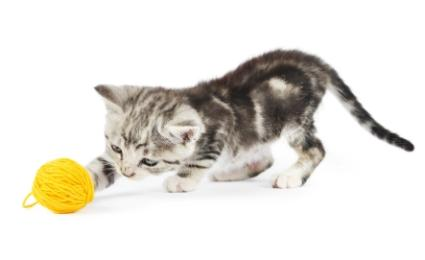
\includegraphics[width=3cm]{../../img/yarn-cat.jpg} \\
  \vspace{1cm}
  \url{http://plato42.stanford.edu/naturalli}
\end{center}
\end{frame}


\end{document}
